\documentclass[12pt,oneside]{article}

%%%%%%%%%%%%%%%%%%%%%%%%%%%%
%%   Zusaetzliche Pakete  %%
%%%%%%%%%%%%%%%%%%%%%%%%%%%%
\usepackage{acronym}
\usepackage{enumerate}
\usepackage{a4wide}
\usepackage{fancyhdr}
\usepackage[pdftex]{graphicx}
\usepackage{palatino}
\usepackage{blindtext}
\usepackage{multirow}
\usepackage[ruled,longend]{algorithm2e}
\usepackage{float}
\usepackage{amsmath}
\usepackage{amssymb}
\usepackage{listings}
\usepackage[numbib]{tocbibind}

%folgende Zeile auskommentieren für englische Arbeiten
\usepackage[ngerman]{babel}

%folgende zeile auskommentieren und die darunter verwenden, um die link-border zu verbergen
\usepackage[bookmarks]{hyperref}
%\usepackage[bookmarks,hidelinks]{hyperref}
\usepackage[T1]{fontenc}
\usepackage[utf8]{inputenc}
\usepackage[a-1b]{pdfx}
\usepackage[justification=centering]{caption}
%\usepackage[style=unsrt,natbib=true,backend=biber]{biblatex}
\usepackage{csquotes}
\usepackage{url}
%\usepackage{subfigure}
\usepackage[utf8]{inputenc}
\usepackage[T1]{fontenc}
% Layout corrections (Schusterjungen)
\clubpenalty = 10000
% Layout corrections (Hurenkinder)
\widowpenalty = 10000
\displaywidowpenalty = 10000

% Figures
\usepackage{caption}
\usepackage[hypcap=true,labelformat=simple]{subcaption}
\renewcommand{\thesubfigure}{(\alph{subfigure})}

% Tables
\usepackage{booktabs}

% Newcommand TODO (red in text)
\newcommand{\todo}[1]{\textcolor{red}{TODO: #1}}

% Newcommand TODOM (red at border)
\newcommand{\todom}[1]{\marginpar{\parbox{1.5cm}{\textcolor{red}{TODO:\\ #1}}}}

% Format für dd.mm.yyy format
\newcommand{\todayddmmyyyy}{%
    \ifnum
        \day<10 0
    \fi\the\day.%
    \ifnum
        \month<10 0
    \fi\the\month.%
    \the\year}


%%%%%%%%%%%%%%%%%%%%%%%%%%%%%%
%% Definition der Kopfzeile %%
%%%%%%%%%%%%%%%%%%%%%%%%%%%%%%

\pagestyle{fancy}
\fancyhf{}
\cfoot{\thepage}
\setlength{\headheight}{16pt}

%%%%%%%%%%%%%%%%%%%%%%%%%%%%%%%%%%%%%%%%%%%%%%%%%%%%%
%%  Definition des Deckblattes und der Titelseite  %%
%%%%%%%%%%%%%%%%%%%%%%%%%%%%%%%%%%%%%%%%%%%%%%%%%%%%%

\newcommand{\HSFTitle}[8]{

    \thispagestyle{empty}
    \begin{center}
    
\includegraphics[width=0.9\textwidth]{logo_new_2.png} \\
    \vspace*{\stretch{1}}
    \end{center}

    %\vspace*{\stretch{1}}
    {\parindent0cm
    \rule{\linewidth}{.7ex}}
    \begin{center}
    \vspace*{\stretch{1}}
    \sffamily\bfseries\Huge
    #1\\
    \vspace*{\stretch{1}}
    \sffamily\bfseries\large
    #3
    \vspace*{\stretch{1}}
    \end{center}
    \rule{\linewidth}{.7ex}

    \vspace*{\stretch{2}}
    \begin{center}
    \Large #2 am #5 der HS Fulda \\
    \vspace*{\stretch{1}}

    \large Matrikelnummer: #4 \\[1mm]
    \large Erstbegutachtung: #7 \\[1mm]

    \vspace*{\stretch{1}}
    \large Eingereicht am #6
    \end{center}
}


%%%%%%%%%%%%%%%%%%%%%%%%%%%%
%%  Beginn des Dokuments  %%
%%%%%%%%%%%%%%%%%%%%%%%%%%%%

\begin{document}

    \HSFTitle
    {Dokumentation und Versionskontrolle in der Softwareentwicklung bei Grenzebach BSH}        % Titel der Arbeit
    {Hausarbeit} % Typ der Arbeit
    {Luca Michael Schmidt}          % Vor- und Nachname der Autor*in
    {1540963}
    {Fachbereich AI}  % Name des FBs
    {\todayddmmyyyy}        % Tag der Abgabe
    {Prof. Dr.-Ing. J. Konert}     % Name der Erstgutachter*in

    \clearpage

    \lhead{}
    \pagenumbering{Roman}
    \setcounter{page}{1}

    \newpage
\begin{otherlanguage}{ngerman}
\thispagestyle{empty}
\section*{Sperrvermerk}
\thispagestyle{empty}
Die vorliegende Arbeit beinhaltet interne vertrauliche Informationen der Firma ”Gren-
zebach BSH GmbH”. Die Weitergabe des Inhalts der Arbeit und Daten im Gesamten
oder in Teilen ist grundsätzlich untersagt.
Es dürfen keinerlei Kopien oder Abschrif-
ten - auch in digitaler Form - gefertigt werden.
Ausnahmen bedürfen der schriftlichen
Genehmigung der Firma Grenzebach BSH GmbH.
\vspace{4\baselineskip}\\
\end{otherlanguage}

    \clearpage
    \tableofcontents
    \clearpage


%%%%%%%%%%%%%%%%%%%%%%%%%%%%
%%  Einstellungen  %%
%%%%%%%%%%%%%%%%%%%%%%%%%%%%
    \cleardoublepage
    \pagenumbering{arabic}
    \setcounter{page}{1}
    \lhead{\nouppercase{\leftmark}}

%%%%%%%%%%%%%%%%%%%%%%%%%%%%
%%  Hauptteil  %%
%%%%%%%%%%%%%%%%%%%%%%%%%%%%

%% ---- %%


    \section{Einleitung}
    \label{sec:einleitung}

    \subsection{Relevanz von Dokumentation und Versionskontrolle}
    \label{subsec:relevanz}
    Die systematische Dokumentation und konsequente Versionskontrolle sind essenzielle Bestandteile moderner Softwareentwicklung. Sie erhöhen die Effizienz von Entwicklungsteams, verbessern die Softwarequalität und ermöglichen eine langfristige Planbarkeit von Wartung und Weiterentwicklung.
    Eine aktuelle und verständliche Dokumentation reduziert den Zeitaufwand für die Informationssuche und beugt Fehlern vor, die zu unerwartetem Mehraufwand führen können \cite{webmakers2024}.
    Dokumentierte Anforderungen dienen als Diskussions- und Entscheidungsgrundlage und fördern die Kommunikation im Team, insbesondere in agilen Kontexten \cite{fraunhoferIESE2020}.
    Die Versionskontrolle sichert den aktuellen Arbeitsstand und ermöglicht durch Branching und Merging eine parallele Feature-Entwicklung, wodurch der Entwicklungsprozess beschleunigt wird \cite{moldstud2024}.
    Teams, die Versionskontrollsysteme effektiv nutzen, produzieren tendenziell weniger Fehler und beheben diese schneller.
    In Kontexten mit schnellen Iterationen und kontinuierlicher Auslieferung sind diese Praktiken unverzichtbar, da sie Stabilität und Nachvollziehbarkeit gewährleisten.

    \subsection{Unternehmenskontext: Grenzebach BSH im Überblick}
    \label{subsec:unternehmenskontext}
    Die Grenzebach BSH GmbH mit Sitz in Bad Hersfeld ist Teil der international agierenden Grenzebach-Gruppe.
    Das 1960 gegründete Unternehmen ist ein globaler Spezialist für Anlagenbau und Automatisierungstechnik. Es beschäftigt weltweit rund 1.600 Mitarbeiter an sieben Standorten und ist in über 55 Ländern aktiv \cite{GrenzebachWebsite}.
    Grenzebach BSH entwickelt und fertigt schwerpunktmäßig Industrieanlagen für die Baustoffe Gips und Holz.
    Neben der in diese Anlagen integrierten Steuerungssoftware gewinnt die Entwicklung von Softwareerweiterungen, spezialisierten Industrie-Apps und unterstützenden Softwarelösungen zunehmend an Bedeutung.
    Die Dokumentations- und Versionsverwaltungsprozesse für diese Softwareentwicklungsprojekte stehen im Zentrum dieser Arbeit.

    \subsection{Zielsetzung und Aufbau der Arbeit}
    \label{subsec:zielsetzung}
    Bei Grenzebach BSH bestehen Optimierungspotenziale in den Prozessen der Dokumentation und Versionskontrolle. Diese Hausarbeit analysiert die gegenwärtigen Praktiken, identifiziert Schwachstellen und entwickelt konkrete Handlungsempfehlungen.
    \newline
    Die Arbeit ist wie folgt aufgebaut:
    Kapitel \ref{sec:grundlagen} legt die theoretische Basis mit grundlegenden Konzepten, Methoden und aktuellen Standards der Dokumentation und Versionskontrolle.
    Anschließend erfolgt eine detaillierte Ist-Analyse bei Grenzebach BSH.
    Kapitel \ref{sec:analyse_dokumentation} untersucht die Dokumentationspraxis, während Kapitel \ref{sec:evaluation_versionskontrolle} die Versionskontrollprozesse evaluiert. Beide Kapitel identifizieren Stärken und Schwächen und vergleichen die Praktiken mit Branchenstandards.
    Darauf aufbauend präsentiert Kapitel \ref{sec:optimierung} spezifische Optimierungsvorschläge und Handlungsempfehlungen.
    Abschließend fasst Kapitel \ref{sec:fazit} die wesentlichen Ergebnisse zusammen, reflektiert diese kritisch und gibt einen Ausblick auf mögliche nächste Schritte.

%% ---- %%


    \section{Theoretische Grundlagen}
    \label{sec:grundlagen}
    Dieses Kapitel erläutert die zentralen Konzepte, Methoden und Werkzeuge der Softwaredokumentation und Versionskontrolle als Fundament für die spätere Analyse und Entwicklung von Optimierungsvorschlägen.

    \subsection{Dokumentation in der Softwareentwicklung}
    \label{subsec:dokumentation}
    Die Softwaredokumentation umfasst alle schriftlichen und grafischen Materialien, die während des Softwarelebenszyklus erstellt werden. Sie beschreibt das Softwaresystem, dessen Entwicklungsprozess und Nutzung.
    Als integraler Bestandteil der Softwareentwicklung ist sie entscheidend für Erfolg, Qualität und langfristige Wartbarkeit.
    Zu den primären Zielen zählen: effektive Kommunikation innerhalb des Teams und mit externen Stakeholdern, strukturierte Wissensspeicherung für Teamwechsel und Onboarding sowie Qualitätssicherung durch klare Spezifikationen und nachvollziehbare Entwicklungsschritte \cite{webmakers2024}.
    Zusätzlich unterstützt sorgfältige Dokumentation die Wartung und Weiterentwicklung bestehender Systeme und erfüllt vertragliche oder regulatorische Anforderungen.
    \newline
    Grundsätzlich unterscheidet man zwischen Prozess- und Produktdokumentation. Die Prozessdokumentation beschreibt den Entwicklungsprozess selbst (z.B. Projektpläne, Meeting-Protokolle). Die Produktdokumentation fokussiert sich auf das zu erstellende oder erstellte Softwaresystem und umfasst verschiedene Artefakte:
    \begin{itemize}
        \item \textbf{Anforderungsdokumentation:} Definiert funktionale Anforderungen durch User Stories oder Use-Case-Diagramme. In agilen Umfeldern ist sie entscheidend zur Vermeidung von Missverständnissen und zur Entwicklung einer gemeinsamen Produktvision \cite{fraunhoferIESE2020}.
        \item \textbf{Architektur- und Design-Dokumentation:} Beschreibt die Systemstruktur, Komponenten und deren Zusammenspiel sowie Entwurfsentscheidungen als Implementierungsleitfaden.
        \item \textbf{Quellcode-Dokumentation:} Umfasst Code-Kommentare und automatisch generierbare API-Dokumentationen für besseres Verständnis einzelner Module und Funktionen.
        \item \textbf{Testdokumentation:} Beinhaltet Testpläne, Testfallspezifikationen, Testdaten und Testprotokolle zur systematischen Qualitätsüberprüfung.
        \item \textbf{Benutzerdokumentation:} Erklärt Endanwendern die Bedienung und Funktionalität durch Handbücher, Online-Hilfen oder Tutorials.
        \item \textbf{Betriebsdokumentation:} Enthält Informationen für Installation, Konfiguration und laufenden Betrieb der Software.
    \end{itemize}
    Typische Herausforderungen sind die kontinuierliche Aktualisierung bei sich entwickelnden Systemen, die Balance zwischen zu viel und zu wenig Dokumentation sowie die Förderung von Akzeptanz und konsequenter Nutzung \cite{webmakers2024}.
    Qualitativ hochwertige Dokumentation zeichnet sich durch klare Struktur, zielgruppengerechte Inhalte und Prozesse zur Qualitätssicherung aus.
    Die ISO/IEC/IEEE 26514 betont dabei die Notwendigkeit von Zielgruppen- und Tätigkeitsanalysen sowie zielgruppenzentrierten Informationskonzepten \cite{styrz2022normen}.

    \subsection{Versionskontrollsysteme und -prozesse}
    \label{subsec:versionskontrolle}
    Ein Versionskontrollsystem (VCS) ist ein fundamentales Werkzeug der Softwareentwicklung. Es protokolliert und verwaltet Änderungen an Dateien systematisch über die Zeit. Der VCS-Einsatz ist unerlässlich für effektive Teamkoordination, lückenlose Änderungshistorie und Quellcode-Integrität \cite{ChaconStraubProGit}. Ohne VCS drohen unbeabsichtigtes Überschreiben von Änderungen, Schwierigkeiten beim Zusammenführen von Arbeitsständen oder unwiderruflicher Verlust funktionierender Versionen \cite{moldstud2024}.
    \newline
    Moderne VCS basieren auf Kernkonzepten mit essenziellen Funktionalitäten. Das Repository speichert alle Projektdateien mit vollständiger Historie. Jede gesicherte Änderung heißt Commit und umfasst geänderte Dateien, Metadaten (Autor, Zeitpunkt) sowie eine erläuternde Commit-Nachricht. Branches ermöglichen parallele Arbeit an Features, isolierte Fehlerbehebung oder Experimente ohne direkten Eingriff in den Hauptzweig (\texttt{main} oder \texttt{master}). Die Integration verschiedener Branches erfolgt durch Merge-Vorgänge. Tags markieren spezifische Stände für Releases. Diffs visualisieren Versionsunterschiede, und Rollbacks ermöglichen die Rückkehr zu früheren Ständen.
    \newline
    Der Git-Arbeitszyklus umfasst typischerweise: initiales Kopieren eines Remote-Repositories (\texttt{git clone}), Vorbereiten geänderter Dateien (Staging mit \texttt{git add}), lokales Speichern als Commit (\texttt{git commit}), Übertragen an Remote-Repository (\texttt{git push}) und Abrufen sowie Integrieren von Remote-Änderungen (\texttt{git pull} oder \texttt{git fetch} mit \texttt{git merge}).

    \subsection{Aktuelle Standards und Best Practices in der Industrie}
    \label{subsec:standards}
    Die Industrie hat diverse Standards und Best Practices entwickelt, um Dokumentation und Versionskontrolle optimal zu nutzen.
    \newline
    Moderne Dokumentationsansätze zielen auf Flexibilität, Aktualität und bessere Prozessintegration. Agile Dokumentationsprinzipien betonen ``gerade genug'' Dokumentation mit Fokus auf funktionierende Software und direkte Kommunikation. User Stories mit präzisen Akzeptanzkriterien spielen oft eine zentrale Rolle \cite{AgileManifestoDe, fraunhoferIESE2020agilMytho}.
    ``Documentation as Code'' behandelt Dokumentation wie Softwarequellcode: Sie wird in Markup-Sprachen (z.B. Markdown, AsciiDoc) verfasst, im VCS gespeichert, durchläuft Review-Prozesse und kann automatisiert in verschiedene Formate überführt werden \cite{WriteTheDocsWhatIsDocsAsCode}.
    \newline
    Für Versionskontrollsysteme, insbesondere Git, haben sich etablierte Praktiken durchgesetzt.
    Dies beginnt bei geeigneten Branching-Modellen wie dem strukturierten Gitflow oder dem agileren Trunk-Based Development \cite{AtlassianGitWorkflows}.
    Standardisierte Commit-Nachrichten nach ``Conventional Commits'' sorgen für klare, maschinell auswertbare Historie \cite{ConventionalCommitsOrgDe}.
    Die Qualitätssicherung erfolgt durch Code Reviews mittels Pull-Requests und transparente Versionierung durch Semantic Versioning (\texttt{MAJOR.MINOR.PATCH}) \cite{AtlassianWasIstEinPullRequest, SemVerOrgDe}.
    Die Integration in CI/CD-Pipelines ermöglicht effiziente und zuverlässige Softwareauslieferung.

    \subsection{Relation zwischen Dokumentation und Versionskontrolle}
    \label{subsec:relation}
    In der modernen Softwareentwicklung sind Dokumentation und Versionskontrolle eng verzahnt und entfalten erhebliche Synergien. Die Verwaltung von Dokumentationsartefakten mittels VCS ist besonders für den ``Documentation as Code''-Ansatz relevant. Textbasierte Dokumente werden gemeinsam mit dem Quellcode versioniert. Durch Branching und Merging können Dokumentationsänderungen parallel zu Code-Features entwickelt und mittels Pull-Requests gemeinsam reviewed werden, was Konsistenz und Nachvollziehbarkeit sicherstellt.
    \newline
    Aussagekräftige Commit-Nachrichten, idealerweise nach Standards wie ``Conventional Commits'' \cite{ConventionalCommitsOrgDe}, dienen als granulare Dokumentation der Änderungshistorie. Moderne Entwicklungsplattformen ermöglichen die Verknüpfung von Dokumentation mit spezifischen Features oder Issues, was das Auffinden kontextbezogener Informationen erleichtert.
    \newline
    Die integrierte Nutzung verbessert Wartbarkeit, Qualität und Transparenz von Softwareprojekten und erleichtert das Onboarding. VCS-gestützte Prozesse, bei denen Dokumentationsanpassungen im selben Zyklus wie Code-Änderungen behandelt werden, meistern die Herausforderung der Synchronisation zwischen dynamischem Code und aktueller Dokumentation.


%% ---- %%


    \section{Analyse der Dokumentationspraxis bei Grenzebach BSH}
    \label{sec:analyse_dokumentation}
    Dieses Kapitel untersucht detailliert die aktuelle Praxis der Erstellung, Verwaltung und Nutzung von Softwaredokumentation bei Grenzebach BSH. Ziel ist ein klares Bild der etablierten Prozesse und eingesetzten Werkzeuge zur Identifikation von Stärken, Schwächen und Optimierungspotenzialen.

    \subsection{Aktuelle Vorgehensweisen und Werkzeuge}
    \label{subsec:dokument_werkzeuge}
    Die Dokumentationspraxis für Softwareprojekte bei Grenzebach BSH basiert auf einer Kombination aus Confluence für übergreifende Projektinformationen und GitHub für technische sowie code-nahe Dokumentation. Diese Zweiteilung richtet sich primär an interne Entwicklerteams.
    \newline
    Für übergeordnete und konzeptionelle Dokumentation neuer Projekte werden Projektseiten in Confluence nach standardisierten Vorlagen angelegt. Diese dienen als zentrale Ablage für verschiedene Artefakte: textuelle Beschreibungen, DrawIO-Grafiken und -Diagramme, Screenshots, Click-Dummies, Prototypen, Wireframes, Interface-Spezifikationen und Besprechungsnotizen. Die kollaborative Erstellung und Pflege erfolgt durch mehrere Teammitglieder. Das jeweils verantwortliche Mitglied sichert Richtigkeit und Qualität durch Proofreading. Die Dokumentation ist regelmäßiger Bestandteil wöchentlicher Scrum-Meetings, in denen Verbesserungen und Aktualisierungen diskutiert werden.
    \newline
    Die technische Dokumentation ist eng mit GitHub und den CI/CD-Prozessen via GitHub Actions verknüpft. Jedes Projekt pflegt einen spezifischen ``Doc-Branch'' im Repository mit HTML-Dateien und eingebundenen JSON-Daten als generierte technische Dokumentation. \texttt{README.md}-Dateien mit grundlegenden Projektinformationen (Zweck, Nutzung, Installation, Besonderheiten) werden nach Vorlage erstellt, ins HTML-Format überführt und integriert. GitHub Actions aktualisieren automatisch Badges in \texttt{README.md}-Dateien für Versionsstand, Testergebnisse und Sicherheitsstatus. Die generierte Dokumentation, die auch extrahierte Code-Kommentare und Kontext aus dem Quellcode umfasst, wird auf einem internen Server publiziert. Bei komplexen Sachverhalten verlinkt sie direkt zu detaillierteren Confluence-Seiten. Die Code-Kommentierung durch Entwickler bildet stets die grundlegendste Dokumentationsebene.
    \newline
    Grenzebach BSH verfolgt einen zweigeteilten Ansatz: Confluence als Wissensbasis für umfassende, grafisch-konzeptionelle Projektinformationen, die kollaborativ erstellt und regelmäßig besprochen werden. GitHub als Zentrum für technische, versionskontrollierte Dokumentation, die teilweise automatisiert generiert, durch CI/CD aktuell gehalten und bei Bedarf mit Confluence verknüpft wird.

    \subsection{Stärken und Schwächen der bisherigen Praxis}
    \label{subsec:ss_dok}
    Die Dokumentationspraxis bei Grenzebach BSH weist sowohl unterstützende Stärken als auch Bereiche mit erkennbaren Herausforderungen und Optimierungspotenzialen auf.
    \newline
    Zu den Stärken zählt die klare Aufgabenteilung zwischen Confluence für übergreifende Informationen und GitHub für code-nahe Dokumentation. Confluence dient als zentrale Ablage für modulübergreifende Artefakte. Die Verwendung von Vorlagen in Confluence ist ein erster Schritt zu mehr Einheitlichkeit. Die automatische HTML-Generierung und Status-Badge-Integration in \texttt{README.md}-Dateien bietet Entwicklern eine schnell erfassbare Projektübersicht. Das Team ist bestrebt, diese Indikatoren positiv zu halten. Die Verlinkungsmöglichkeit von Code-Kommentaren zu erläuternden Confluence-Inhalten wird als hilfreich für das Verständnis komplexer Zusammenhänge empfunden.
    \newline
    Demgegenüber stehen Schwächen und Herausforderungen. Die Aufteilung auf Confluence und GitHub führt trotz Verlinkungen zu potenziellen Problemen ohne automatisierte Synchronisation. Dies kann Inkonsistenzen verursachen: veraltete Code-Kommentare, \texttt{README.md}-Dateien oder Confluence-Seiten sowie tote Links \cite{webmakers2024}. Klare Regeln zur führenden Informationsquelle fehlen, wobei tendenziell Confluence für allgemeine und GitHub für code-spezifische Informationen genutzt wird. Die Qualität der Code-Kommentare variiert stark je nach Teammitglied. Obwohl Confluence-Seiten generell gut gepflegt sind, bleibt die kontinuierliche Aktualisierung eine Herausforderung. Die Dokumentationsthematisierung in Scrum-Meetings fokussiert häufiger auf Tests. Nicht alle Teammitglieder zeigen gleiches Engagement für Dokumentationsaufgaben. Wichtige Aspekte werden teilweise auch auf Rückfrage nicht ergänzt. Eine vollständige Abdeckung aller Dokumentationsarten (siehe \ref{subsec:dokumentation}), insbesondere für Endanwender, fehlt, während andere Bereiche gut abgedeckt sind.

    \subsection{Vergleich mit Branchenstandards}
    \label{subsec:vergleich_dok}
    Der Vergleich mit den Branchenstandards aus Kapitel \ref{sec:grundlagen} zeigt sowohl fortschrittliche Ansätze als auch Weiterentwicklungspotenziale.
    \newline
    Positiv sind die GitHub-Actions-basierte HTML-Generierung, die Versionierung im ``Doc-Branch'' und die Code-Kommentar-Extraktion hervorzuheben. Diese Aspekte implementieren Elemente des ``Documentation as Code''-Prinzips \cite{WriteTheDocsWhatIsDocsAsCode}. Die automatische Generierung aus dem reviewten \texttt{develop}-Branch ohne manuelle Überarbeitung fördert Konsistenz. Die Nutzung von \texttt{README.md}-Dateien mit automatisierten Status-Badges entspricht modernen Praktiken. Die Dokumentationsbesprechung in Scrum-Meetings unterstützt agile Grundsätze \cite{AgileManifestoDe, fraunhoferIESE2020agilMytho}. Die einheitliche DrawIO-Nutzung für Confluence-Diagramme ist ebenfalls positiv.
    \newline
    Optimierungspotenzial zeigt sich in der Durchgängigkeit des ``Documentation as Code''-Ansatzes. Werkzeuge, die Markdown oder AsciiDoc direkt aus dem Haupt-Repository verarbeiten (wie Sphinx oder MkDocs), könnten den separaten ``Doc-Branch'' reduzieren und eine engere Code-Verzahnung ermöglichen. Dies würde Review-Prozesse vereinfachen, da Dokumentationsänderungen im selben Diff wie Code-Änderungen sichtbar wären. Die HTML-Bereitstellung auf einem internen Webserver ist funktional, könnte aber durch integrierte GitHub-Wiki-Funktionen oder spezialisierte Doku-Hosting-Plattformen optimiert werden.
    \newline
    Die Trennung auf Confluence und GitHub-generierte Seiten weicht potenziell vom ``Single Source of Truth''-Ideal ab ohne klare Prozesse für führende Quellen und Aktualitätssicherung \cite{webmakers2024}. Die variierende Dokumentationsqualität je nach Teammitglied deutet auf fehlende verbindliche Richtlinien hin. Eine systematische Qualitätssicherung über Proofreading hinaus, orientiert an ISO/IEC/IEEE 26514 \cite{styrz2022normen}, fehlt noch. Eine automatisierte Verlinkungsprüfung zwischen Confluence und GitHub wäre eine Annäherung an Best Practices für wartbare Dokumentationssysteme.

%% ---- %%


    \section{Evaluation der Versionskontrolle bei Grenzebach BSH}
    \label{sec:evaluation_versionskontrolle}
    Nach der Dokumentationsanalyse widmet sich dieses Kapitel der detaillierten Evaluation der Versionskontrollsysteme und zugehörigen Workflows bei Grenzebach BSH. Ziel ist die Beschreibung aktueller Prozesse, Identifikation von Stärken und Schwächen sowie der Vergleich mit Branchenstandards.

    \subsection{Eingesetzte Versionskontrollsysteme und Workflows}
    \label{subsec:vk_systeme}
    Die Versionskontrolle basiert auf Git mit GitHub als zentraler Hosting-Plattform. Ergänzend kommen GitHub Actions für CI/CD und Jira für das Projektmanagement zum Einsatz. Spezielle Git-Clients über die IDE-integrierten Funktionen (JetBrains, Visual Studio Code) hinaus werden nicht verwendet. Die Git- und GitHub-Nutzung ist im Team etabliert und wird wie vorgesehen umgesetzt.
    \newline
    Die Projekterstellung folgt einem standardisierten Prozess: Ein Git-Template wird heruntergeladen und ein Setup-Skript ausgeführt. Dies generiert die Git-Umgebung, erstellt das GitHub-Repository mit Zugriffsrechten, legt einen ``Doc-Branch'' an, richtet GitHub Actions ein und passt \texttt{README.md} sowie Standarddateien (\texttt{.gitignore}, \texttt{LICENSE}) an. Dieser Ablauf funktioniert reibungslos und spart Zeit bei der Projekteinrichtung.
    \newline
    Das Branching-Modell ist klar definiert und wird konsequent eingehalten. Der \texttt{develop}-Branch ist der Hauptentwicklungszweig. Feature-Branches folgen dem Schema \texttt{GBV-xxx} und beziehen sich auf Jira-Tickets. Releases werden durch Tags im Format \texttt{vx.x.x} markiert. Diese werden manuell gesetzt, woraufhin die CI/CD-Pipeline deren Validität prüft und einen formalen GitHub-Release erstellt.
    \newline
    Pull Requests (PRs) sind zentraler Workflow-Bestandteil. Änderungen aus Feature-Branches werden nicht direkt gemerged, sondern durchlaufen einen PR-Prozess. Der Feature-Entwickler initiiert den PR, der ein Code-Review durch mindestens einen Kollegen erfordert, typischerweise jemand mit Feature-Kenntnis. Nach Zustimmung erfolgt der Merge in \texttt{develop}. Dieser Prozess wird konsequent befolgt.

    Abbildung \ref{fig:git_workflow} visualisiert den beschriebenen Git-Workflow mit dem etablierten Branching-Modell und dem integrierten Review-Prozess.

    \begin{figure}[H]
        \centering
        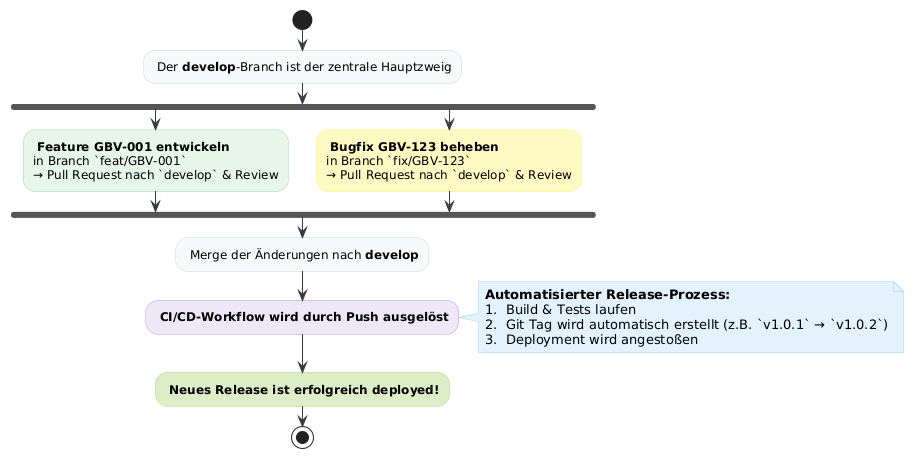
\includegraphics[width=0.85\textwidth]{images/git_branching}
        \caption{Git-Workflow bei Grenzebach BSH: Feature- und Bugfix-Branches (GBV-xxx) durchlaufen einen Pull-Request-Prozess mit Review vor dem Merge in develop. Ein Push auf develop löst automatisch den CI/CD-Workflow und Release-Prozess aus}
        \label{fig:git_branching}
    \end{figure}
    \noindent
    Die CI via GitHub Actions ist an Commits auf \texttt{develop} gekoppelt. Die Pipeline umfasst: Projektinformationsextraktion und \texttt{README.md}-Aktualisierung, Code-Linting und -Formatierung, Sicherheitsprüfung, automatisierte Tests und Dokumentationsgenerierung mittels \texttt{pdoc}. CI-Rückmeldungen sind meist zielführend; bei komplexen Fehlern ist der Pipeline-Verantwortliche zuständig.
Die konkrete Ausgestaltung der CI/CD-Pipeline mit allen automatisierten Schritten und deren Abhängigkeiten zeigt Abbildung \ref{fig:git_workflow}.

    \begin{figure}[H]
        \centering
        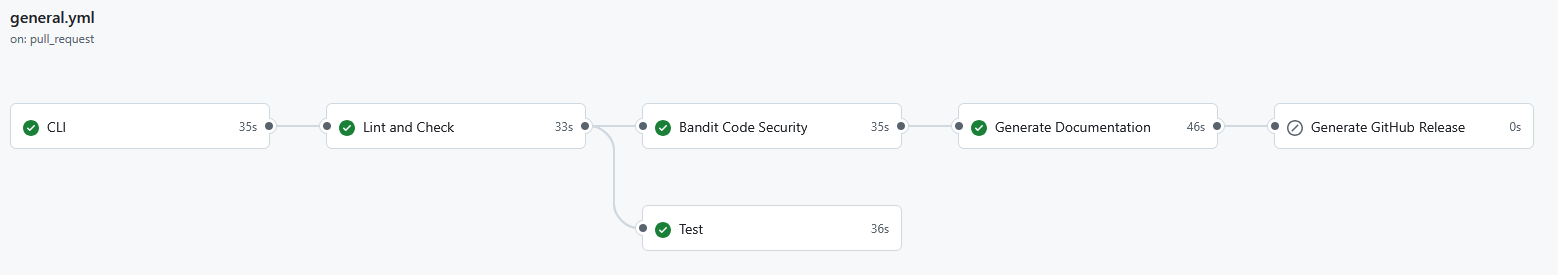
\includegraphics[width=0.9\textwidth]{images/git_workflow}
        \caption{GitHub Actions CI/CD-Pipeline (general.yml) bei Grenzebach BSH: Sequenzielle Ausführung von CLI-Checks, Code-Linting, Sicherheitsprüfung mit Bandit, Tests und Dokumentationsgenerierung mit finaler Release-Erstellung}
        \label{fig:git_workflow}
    \end{figure}

    \noindent
    Die CD erfolgt ebenfalls über GitHub Actions nach erfolgreichem \texttt{develop}-Push und beinhaltet das Deployment auf einen internen Server. Nach Release-Tag-Erstellung wird die Software auf einem internen PyPi-Server bereitgestellt. Dieser aktualisiert sich selbstständig, was GitHub-unabhängige Bibliotheksinstallationen ermöglicht.
    \newline
    Die Jira-Verknüpfung erfolgt primär über Branch-Benennung nach Ticketnummern (\texttt{GBV-xxx}), was die Nachverfolgbarkeit erleichtert. Eine automatisierte Jira-GitHub-Synchronisation (z.B. automatische Kommentare oder Statusänderungen) ist nicht implementiert; die Information über PRs erfolgt manuell.

    \subsection{Stärken und Schwächen der aktuellen Prozesse}
    \label{subsec:ss_vk}
    Die Analyse der Versionskontrollprozesse zeigt Stärken, die zu effizienter und qualitativ hochwertiger Entwicklung beitragen, aber auch Optimierungsbereiche.
    \newline
    Wesentliche Stärken sind die konsequente Git- und GitHub-Nutzung als zentrale Plattform. Der GitHub-Funktionsumfang, insbesondere CI/CD über GitHub Actions mit eigenen Unternehmens-Runnern, wird als vorteilhaft und kosteneffizient empfunden. Die gute Git-Integration in IDEs unterstützt einen reibungslosen Workflow. Der standardisierte Projekterstellungsprozess mittels Templates und Setup-Skripten spart Zeit und sorgt für konsistente Projektstrukturen, primär für Python-Projekte. Das etablierte Branching-Modell mit klarer Trennung von Entwicklungs-, Feature- und Release-Zweigen fördert stabiles Release-Management und organisierte Feature-Entwicklung.
    \newline
    Die weitgehende CI/CD-Automatisierung ist eine weitere Stärke. Automatisierte Tests, Linting und Security Checks erhöhen die Code-Qualität und geben frühes Feedback. Die automatische Dokumentationsgenerierung und \texttt{README.md}-Aktualisierung mit Status-Badges erhöht Transparenz und Aktualität wichtiger Projektinformationen. Der obligatorische PR-Prozess mit Code-Review ist ein wichtiger Qualitätssicherungs- und Wissenstransfermechanismus. Entwickler fühlen sich durch VCS-Prozesse und Automatisierung gut unterstützt, während die CI/CD-Wartung bei einem dedizierten Entwickler liegt.
    \newline
    Trotzdem existieren Schwächen und Herausforderungen. Das Debugging von GitHub-Actions-Fehlern kann komplex und zeitaufwendig sein. Die Test-Ausführungsgeschwindigkeit könnte durch stärkere Parallelisierung verbessert werden, wofür jedoch zeitliche Ressourcen fehlen. Strenge Linting-Regeln werden gelegentlich als hinderlich empfunden, obwohl sie grundsätzlich positiv für die Code-Qualität sind.
    \newline
    Bei Code-Reviews findet zwar ein Review statt, formalisierte Richtlinien oder Checklisten fehlen jedoch (außer erfolgreicher CI-Pipeline). Dies kann zu variierender Review-Tiefe führen. Für kritische Änderungen könnte ein einzelner Reviewer unzureichend sein. Die Commit-Nachrichten-Qualität ist mittelmäßig ohne verbindliche Regeln, was zu vagen Nachrichten oder umfangreichen Commits führt.
    \newline
    Die fehlende tiefere Jira-GitHub-Integration ist ein Schwachpunkt. Automatisches Ticket-Schließen bei gemergten PRs oder ``tote Link''-Erkennung wären wünschenswerte Verbesserungen.

    \subsection{Vergleich mit Branchenstandards}
    \label{subsec:vergleich_vk}
    Der Abgleich mit den Branchenstandards aus Abschnitt \ref{subsec:standards} ermöglicht weitere Einordnung und zeigt Entwicklungsmöglichkeiten.
    \newline
    Das Branching-Modell kombiniert Elemente von Gitflow und Trunk-Based Development. Die Trennung zwischen \texttt{develop} und Release-Tags ähnelt Gitflow und ermöglicht stabiles Release-Management. Die zeitnahe Feature-Branch-Integration in \texttt{develop} vermeidet langlaufende Zweige, was Trunk-Based Development entspricht \cite{AtlassianGitWorkflows}. Dieser hybride Ansatz funktioniert gut, könnte aber weniger flexibel für extrem schnelle Release-Zyklen sein.
    \newline
    Die ``Conventional Commits''-Prinzipien \cite{ConventionalCommitsOrgDe} werden nicht verbindlich umgesetzt. Entwickler bemühen sich um aussagekräftige Nachrichten, eine einheitliche, maschinell auswertbare Struktur fehlt jedoch. Die Einführung dieses Standards würde die Historie verbessern bei geringem Umstellungsaufwand.
    \newline
    Der Ein-Personen-Code-Review entspricht grundlegenden Best Practices \cite{AtlassianWasIstEinPullRequest}. Branchenstandards empfehlen oft detailliertere Review-Richtlinien und für kritische Änderungen ein Vier-Augen-Prinzip zur Effektivitätssteigerung und Betriebsblindheitsreduzierung.
    \newline
    Die Verwendung von \texttt{vx.x.x}-Tags und bewusste Versionsnummern-Semantik zeigt klare Orientierung am Semantic Versioning \cite{SemVerOrgDe}, was transparente Änderungskommunikation ermöglicht.
    \newline
    Die CI/CD-Integration wird als gut und Best-Practice-konform eingeschätzt. Verbesserungspotenzial wie Test-Workflow-Parallelisierung wurde intern erkannt und entspricht dem Optimierungsgedanken der Branchenstandards.
    \newline
    Grenzebach BSH nutzt GitHub-Kernfunktionen gut aus. Ungenutztes Potenzial besteht bei erweiterten Features: GitHub Projects für integriertere Projektplanung, detaillierte Issue-Templates oder Code-Owner-Features könnten den Workflow optimieren.

%% ---- %%


    \section{Optimierung}
    \label{sec:optimierung}
    Aufbauend auf der Analyse der Dokumentations- und Versionskontrollpraxis (Kapitel \ref{sec:analyse_dokumentation} und \ref{sec:evaluation_versionskontrolle}) sowie dem Branchenstandardvergleich werden konkrete Optimierungsvorschläge und Handlungsempfehlungen vorgestellt. Ziel ist die Adressierung identifizierter Schwachstellen und Steigerung von Effizienz, Qualität und Konsistenz.

    \subsection{Handlungsempfehlungen zur Dokumentation}
    \label{subsec:empfehlungen_dok}
    Die Untersuchung zeigt trotz vorhandener Stärken diverse Optimierungspotenziale. Die nachfolgenden Empfehlungen zielen auf deren Nutzung:

    \subsubsection{Verbesserung der Konsistenz und Verknüpfung zwischen Confluence und GitHub}
    \label{subsubsec:doku_konsistenz_verknuepfung}
    Die Konsistenzgewährleistung zwischen Confluence und GitHub ist durch fehlende automatisierte Verknüpfung herausfordernd. Folgende Maßnahmen werden empfohlen:
    \begin{itemize}
        \item \textbf{Link-Management-Tool einführen:} Ein ``Broken-Link-Checker'' könnte fehlerhafte Verweise frühzeitig identifizieren und die Verlinkungszuverlässigkeit erhöhen.
        \item \textbf{Plugin-Integration verbessern:} Confluence-Plugins wie ``GitHub links for Confluence'' \cite{GitHubLinksForConfluenceMarketplace} sollten für direktere, dynamischere Verknüpfungen evaluiert werden.
        \item \textbf{``Single Source of Truth'' definieren:} Für spezifische Informationstypen sollte die führende Quelle verbindlich festgelegt werden. API-Dokumentationen könnten ausschließlich aus Code generiert werden, während Prozessbeschreibungen in Confluence verbleiben.
    \end{itemize}

    \subsubsection{Stärkung des ``Documentation as Code''-Ansatzes}
    \label{subsubsec:doku_docs_as_code}
    Der etablierte Ansatz der automatisierten technischen Dokumentationsgenerierung ist ein Kernbestandteil der ``Documentation as Code''-Strategie \cite{WriteTheDocsWhatIsDocsAsCode}. Zur weiteren Optimierung:
    \begin{itemize}
        \item \textbf{Generierungs-Tooling optimieren:} Periodische Evaluation, ob \texttt{pdoc} alle Anforderungen erfüllt oder alternative Werkzeuge Vorteile bieten.
        \item \textbf{Workflows modularisieren:} GitHub-Actions-Workflows sollten flexibler gestaltet werden für vereinfachte Projektanpassung und erleichtertes Debugging.
    \end{itemize}
    Da die Dokumentationspflege primär in Code-Kommentaren erfolgt, würde konsequente Kommentarqualitätsverbesserung (siehe \ref{subsubsec:doku_motivation_qualitaet}) Akzeptanz und Nutzen erhöhen.

    \subsubsection{Steigerung der Motivation und Qualität bei der Dokumentationserstellung}
    \label{subsubsec:doku_motivation_qualitaet}
    Die variierende Kommentarqualität und unterschiedliches Engagement deuten auf Motivations- und Verantwortlichkeitsherausforderungen hin:
    \begin{itemize}
        \item \textbf{Klare Verantwortlichkeiten:} Definition von Zuständigkeiten für Confluence-Seiten oder Moduldokumentationen schafft Verbindlichkeit.
        \item \textbf{Sprint-Integration:} Dokumentation sollte feste Aufgabe in Jira-Tickets werden und Teil der ``Definition of Done'' sein.
        \item \textbf{Code-Kommentar-Richtlinien:} Praxisnahe Richtlinien können Konsistenz steigern, da Grundkompetenz vorhanden ist.
        \item \textbf{Effektivere Scrum-Thematisierung:} Ein fester Agenda-Punkt (z.B. ``Doku-Mittwoch'') analog zum ``Test-Montag'' könnte etabliert werden.
    \end{itemize}

    \subsubsection{Verbesserung der Auffindbarkeit und Struktur von Dokumentation}
    \label{subsubsec:doku_auffindbarkeit}
    Gegen erschwerte Informationssuche bei wachsendem Dokumentationsumfang:
    \begin{itemize}
        \item \textbf{Einheitliche Nomenklatur:} Vereinheitlichung von Fachbegriffen über alle Plattformen zur Missverständnisvermeidung.
        \item \textbf{Strukturierungsprinzipien implementieren:} Einheitliche Prinzipien für Confluence und HTML-Dokumentation mit konsequenter Indexierung.
    \end{itemize}

    \subsubsection{Systematische Erstellung von Architektur- und Testdokumentation}
    \label{subsubsec:doku_architektur_test}
    Zur systematischen Erstellung und Pflege wird die Einführung fester Vorlagen analog zu Code-Templates empfohlen. Diese sollten wesentliche Aspekte vorgeben und als Standard etabliert werden.

    \subsection{Optimierungsansätze für die Versionskontrolle}
    \label{subsec:konzepte_vk}
    Trotz solider Grundlage existieren konkrete Ansatzpunkte zur Steigerung von Effizienz, Stabilität und Nutzerfreundlichkeit.

    \subsubsection{Verbesserung der CI/CD-Pipeline-Effizienz und -Wartbarkeit}
    \label{subsubsec:vk_cicd_optimierung}
    Die CI/CD-Prozesse bieten Optimierungspotenzial. Für erleichtertes Debugging empfiehlt sich detaillierteres Logging und Pre-Commit-Hooks für lokale Vorabprüfungen. Modularere GitHub-Actions-Workflows würden Projektanpassbarkeit erhöhen und Wartungsabhängigkeiten reduzieren. Zur Durchlaufzeitenverkürzung sollte zusätzliche Code-Runner für stärkere Parallelisierung evaluiert werden. Caching-Mechanismen oder selektive Testausführung könnten zusätzlich zur Geschwindigkeitssteigerung beitragen.

    \subsubsection{Förderung der Akzeptanz und Effektivität von Code-Qualitätsstandards}
    \label{subsubsec:vk_code_qualitaet}
    Bei als streng empfundenen Regeln sollte der Fokus auf transparenter Vorteilskommunikation liegen, verbunden mit periodischen Team-Überprüfungen. Die verbindliche Einführung von ``Conventional Commits'' \cite{ConventionalCommitsOrgDe} wird empfohlen. Der Schulungsaufwand wäre gering bei IDE-Plugin-Unterstützung, der Nutzen läge in verbesserter Nachvollziehbarkeit und professionellerer Projekthistorie.

    \subsubsection{Stärkung des Code-Review-Prozesses}
    \label{subsubsec:vk_code_review}
    Der aktuelle Review-Prozess kann zur Qualitätssteigerung ausgebaut werden. Review-Checklisten könnten Konsistenz und Gründlichkeit erhöhen. Diese sollten Kernaspekte wie Fehlerfreiheit, Standardkonformität, Lesbarkeit und Testabdeckung umfassen. Für kritische Änderungen sollte das situative Vier-Augen-Prinzip erwogen werden.

    \subsubsection{Optimierung der Werkzeugnutzung und Integrationen}
    \label{subsubsec:vk_tool_integration}
    Es sollte geprüft werden, inwieweit GitHub Apps oder Actions eine stärkere Jira-GitHub-Automatisierung realisieren können: automatische Verlinkung von Commits/PRs in Tickets und Status-Updates. Die Nutzung des GitHub Wikis pro Repository als technische Dokumentationsplattform sollte evaluiert werden, um Dokumentation direkter am Quellcode zu bündeln.

    \subsection{Integrierte Implementierungsstrategie}
    \label{subsec:integration}
    Die erfolgreiche Umsetzung erfordert eine durchdachte Strategie mit Priorisierung, Vorgehensmodell, Verantwortlichkeiten und Erfolgsmessung.
    \newline
    Für die Priorisierung werden ``Quick Wins'' mit hohem Nutzen bei geringem Aufwand empfohlen: verbindliche ``Conventional Commits'', einheitliche Nomenklatur und stärkere Dokumentationsthematisierung in Scrum-Meetings. Mittelfristig sollten aufwändigere Verbesserungen wie GitHub-Actions-Optimierung und verbesserte Confluence-GitHub-Konsistenz angegangen werden. Langfristige Maßnahmen wie weitere Code-Runner oder tiefere Atlassian-Integration könnten nach erfolgreichen ersten Schritten evaluiert werden.
    \newline
    Ein schrittweises Vorgehen mit Pilotprojekten für 1-2 Module minimiert Risiken und ermöglicht Erfahrungssammlung vor vollständigem Rollout. Kontinuierliche Team-Einbindung durch regelmäßige Updates und Feedback-Möglichkeiten ist essenziell für Akzeptanz.
    \newline
    Die Planungsverantwortung sollte beim gesamten Team liegen für breites Commitment. Die Umsetzung einzelner Maßnahmen kann an kompetente oder interessierte Teammitglieder delegiert werden. Interne Workshops und klare Anleitungen sind ausreichend; externe Schulungen scheinen nicht erforderlich.
    \newline
    Zur Erfolgsmessung könnten regelmäßige Team-Umfragen zur Zufriedenheit durchgeführt werden. Quantitativ ließe sich der Erfolg durch Analyse von Workflow-Fehlern bewerten, die auf mangelhafte Dokumentation oder unklare Commits zurückzuführen sind.
    \newline
    Die Umsetzungsplanung kann durch Jira unterstützt werden. Quick Wins sollten innerhalb weniger Wochen umgesetzt werden, mittelfristige Ziele in ein bis zwei Monaten, langfristige Ziele in drei bis sechs Monaten.

%% ---- %%


    \section{Fazit und Ausblick}
    \label{sec:fazit}
    Diese Hausarbeit analysierte die Dokumentations- und Versionskontrollprozesse bei Grenzebach BSH und entwickelte konkrete Optimierungspotenziale sowie Handlungsempfehlungen. Dieses Kapitel fasst die Kernerkenntnisse zusammen, gibt einen Zukunftsausblick und beinhaltet ein persönliches Resümee.

    \subsection{Zusammenfassung der Kernerkenntnisse}
    \label{subsec:zusammenfassung}
    Die Dokumentationspraxis-Untersuchung (Kapitel \ref{sec:analyse_dokumentation}) zeigt eine solide Basis mit erheblichem Optimierungspotenzial. Positiv ist der Ansatz der teilweise automatisierten technischen Dokumentationsgenerierung aus Quellcode mit Integration von Testergebnissen und Sicherheitschecks. Als zentrale Schwachstelle wurde mangelnde Standardisierung bei Erstellung und Pflege identifiziert. Dies zeigt sich in variierender Kommentarqualität und der Notwendigkeit einheitlicherer Vorlagen für Confluence.
    \newline
    Die Versionskontrollevaluation (Kapitel \ref{sec:evaluation_versionskontrolle}) ergab ein sehr solides Bild. Besonders positiv sind etablierte, automatisierte CI/CD-Workflows und die Git-Template-Nutzung für standardisierten Projektstart. Als wesentliche Schwachstelle wurde die fehlende Commit-Nachrichten-Standardisierung identifiziert, was im Kontrast zur erfolgten Branch-Namen-Standardisierung steht.
    \newline
    Die übergeordnete Erkenntnis: Bei Grenzebach BSH existieren gute informationstechnische und prozessuale Grundlagen, die Potenziale könnten jedoch durch stärkere Standardisierung und Maßnahmen zur Motivationssteigerung für Dokumentationsaufgaben besser ausgeschöpft werden.
    \newline
    Zur Schwachstellenadressierung wurden in Kapitel \ref{sec:optimierung} konkrete Empfehlungen entwickelt. Für die Dokumentation: einheitliche Confluence-Vorlagen zur Konsistenzerhöhung und Code-Kommentar-Standardisierung zur Verbesserung von Lesbarkeit und Nachvollziehbarkeit. Für die Versionskontrolle: Commit-Nachrichten-Standardisierung zur Nachvollziehbarkeitssteigerung und CI/CD-Workflow-Weiterentwicklung zur Qualitätssicherungsverbesserung. Diese Maßnahmen zielen auf Effizienzsteigerung, Qualitätssicherung und Prozessoptimierung gemäß der Einleitungszielsetzung.

    \subsection{Zukunftsausblick und persönliches Resümee}
    \label{subsec:zukunft}
    Über die vorgeschlagenen Optimierungsmaßnahmen hinaus ergeben sich weitere Perspektiven für Grenzebach BSH und persönliche Weiterentwicklung.
    \newline
    Nach Umsetzung priorisierter Empfehlungen könnte die Anschaffung zusätzlicher Code-Runner für CI/CD-Pipelines sinnvoll sein. Dies würde stärkere Test-Parallelisierung ermöglichen und die Gesamteffizienz steigern. Eine tiefere Atlassian-Toolchain-Integration bedarf sorgfältiger Team-Evaluation. Technologische Trends wie KI-gestützte Dokumentationswerkzeuge sollten beobachtet werden. Sie könnten Effizienz und Konsistenz erheblich verbessern, bergen aber Risiken bei unsachgemäßer Anwendung. Die bestehenden DevOps-Praktiken könnten durch kontinuierlichen Wissensaufbau und neue Werkzeuge stetig optimiert werden.
    \newlineT
    Persönlich war die tiefgehende Auseinandersetzung mit Dokumentationspraktiken besonders erkenntnisreich. Die unterschiedliche Konsistenz zwischen Entwicklern war mir bewusst, aber erst die Analyse verdeutlichte das volle Ausmaß und deren Einfluss auf die Gesamtqualität. Daraus resultierte die Erkenntnis über die Notwendigkeit, Standards nicht nur zu definieren, sondern deren Umsetzung zu fördern. Bei der Versionskontrolle bestätigte die Analyse die Notwendigkeit der CI/CD-Workflow-Überarbeitung. Die größte Herausforderung bestand darin, komplexe, teils informelle Praktiken vollständig zu erfassen und strukturiert darzustellen.
    \newline
    Die gewonnenen Erkenntnisse schärften meine Sichtweise auf die Bedeutung von Dokumentation und Versionskontrolle. Für meine zukünftige Entwicklertätigkeit werde ich verstärkt auf Standardeinhaltung, Konsistenzförderung und die Betrachtung von Dokumentation als integralen, wertvollen Prozessbestandteil achten, statt sie als nachgelagerte Pflichtübung zu verstehen.


%%%%%%%%%%%%%%%%%%%%%%%%%%%%
%% Werkzeugverzeichnis
%%%%%%%%%%%%%%%%%%%%%%%%%%%%
    \clearpage
    \section{Verzeichnis der verwendeten Werkzeuge}
\label{sec:tools}

% Eigene Umgebung, die wie thebibliography aussieht, aber keine eigene Überschrift hat
\begin{list}{}{%
\setlength{\labelwidth}{1.5cm}%
\setlength{\labelsep}{0.3cm}%
\setlength{\leftmargin}{2cm}%
\setlength{\itemindent}{0cm}%
\setlength{\listparindent}{0cm}%
}

\item[\textbf{[Claude]}] \textbf{Claude} (3.7 Sonnet, Anthropic)\\
\emph{Verwendung:} 
\begin{itemize}
  \item Beihilfe für die Gliederung und Strukturierung der Hausarbeit
  \item Überarbeitung von Formulierungen in: \ref{sec:einleitung}, \ref{sec:grundlagen}, \ref{sec:evaluation_versionskontrolle}
\end{itemize}

\item[\textbf{[Claude]}] \textbf{Claude} (4 Opus, Anthropic)\\
\emph{Verwendung:} 
\begin{itemize}
  \item Rechtschreibprüfung Gesamtdokument
  \item Konsistenzprüfung Gesamtdokument
  \item Quellenprüfung Gesamtdokument
  \item  Korrekturempfehlungen Gesamtdokument
\end{itemize}

\item[\textbf{[Gemini]}] \textbf{Gemini} (Gemini 2.5 Pro, Google)\\
\emph{Verwendung:} 
\begin{itemize}
  \item Beihilfe der Strukturierung von \ref{sec:einleitung}, \ref{sec:optimierung}
  \item Rechtschreibprüfung in: \ref{sec:einleitung}, \ref{sec:grundlagen}, \ref{sec:analyse_dokumentation}, \ref{sec:evaluation_versionskontrolle}, \ref{sec:optimierung}, \ref{sec:fazit}
  \item Literaturempfehlungen
\end{itemize}

\end{list}

%%%%%%%%%%%%%%%%%%%%%%%%%%%%
%% Literaturverzeichnis wird
%% automatisch eingefügt
%%%%%%%%%%%%%%%%%%%%%%%%%%%%
    \clearpage
    \def\UrlBreaks{\do\/\do-} %ermöglicht zeilenumbrüche in URLs im Literaturverzeichnis bei / und -
%\stepcounter{section} % Increase counter (section) by one step
%\addcontentsline{toc}{section}{\thesection \quad Literaturverzeichnis}
    \bibliographystyle{unsrt}
    \bibliography{literatur}
% --------------------------

%\subsection{Erstellung eines PDFs im PDF-A Format}
%Durch Einbinden geeigneter Packages (pdfx) wird diese Vorlage bereits als PDF-A erzeugt. Sie sollten allerdings die Metadaten in der Datei main.xmpdata %anpassen!

    \newpage
\begin{otherlanguage}{ngerman}
\thispagestyle{empty}
\section*{Eidesstattliche Erklärung}
\thispagestyle{empty}
Hiermit versichere ich, die vorliegende Arbeit selbstständig verfasst und keine anderen als die angegebenen Quellen und Hilfsmittel benutzt sowie die Zitate deutlich kenntlich gemacht zu haben.
\newline
Ich erkläre weiterhin, dass die vorliegende Arbeit in gleicher oder ähnlicher Form noch nicht im Rahmen eines
anderen Prüfungsverfahrens eingereicht wurde.
\vspace{4\baselineskip}\\
Bad Hersfeld, den \today \hfill Luca Michael Schmidt
\vspace{4\baselineskip}\\
\end{otherlanguage}

\end{document}
